\documentclass[../../main.tex]{subfiles}

\begin{document}

\section{Introduction}


From \autoref{tab:memory-usage-comparison} and \autoref{tab:memory-usage-comparison-2D}, it is clear that the Transformer models are memory-intensive due to their quadratic complexity in terms of the dataset size. This is a significant bottleneck for scaling up the Transformer models to larger datasets with limited compute resources. To address this issue, several methods have been proposed to reduce the memory complexity of the Transformer models which we will explore in this chapter.

\section{Pseudotokens}

Pseudotokens (also known as Inducing Points) are a set of tokens that are used to approximate the full set of tokens, it can be thought of as a lower dimensional representation of the data set. They have been widely used in the context of Gaussian Processes (GPs) to reduce the complexity of the model with great success \parencite{hensman2013gaussian}. The original tokens $\bm{X} \elof{N}{D}$ are projected onto into a lower-dimensional space $\bm{I} \elof{M}{D}$ where $M << N$ through some translation equivariant network \parencite{anonymous2024translationequivariant} giving us the pseudotokens $\bm{I}$ which are translation equivariant to the original tokens $\bm{X}$. We then perform cross-attention between the pseudotokens $\bm{I}$ and the original tokens $\bm{X}$, hence reducing the memory complexity to $\mathcal{O}(MN_c + MN_t)$. 


% ./fig/set-transformer.png

\begin{figure}[H]
    \centering
    \includegraphics[width=0.9\textwidth]{fig/set-transformer.png}
    \caption{Perceiver vs Set Transformer. MAB is equivalent to Multi-Head Cross Attention, refer to \parencite{jaegle2021perceiver, lee2019set} for more details.}
    \label{fig:set-transformer}
\end{figure}

We consider two implementations of a pseudotokens based Transformer, one is the Set Transformer \parencite{lee2019set} and the other is the Perceiver \parencite{jaegle2021perceiver}. Both models are very similar and differ in the way they implement the cross-attention mechanism between the original and pseudo tokens \autoref{fig:set-transformer}. \cite{feng2023latent} implemented the Perciever model in the context of NPs creating the `Latent Bottled Attention Neural Process' (LBANP) model. \cite{anonymous2024translationequivariant} implemented the Set Transformer model into a NP creating the `Inducing Set Transformer' (IST) model. \cite{anonymous2024translationequivariant} found both models to perform very similarly. Both models will be encompassed under the `PT-TETNP' term in the results' section since they are very similar in terms of performance.

\section{Linear Transformer}

\cite{katharopoulos2020transformers} introduces a kernelized form of the attention mechanism that allows the model to be linear with the number of tokens. The output of an attention head $\bm{H}$ is computed as follows:

\begin{equation}
    \bm{H}_i = \frac{\phi(\bm{Q}_i)^T \sum_{j=1}^{N} \phi(\bm{K}_j) \bm{V}_j^T}{\phi(\bm{Q}_i)^T \sum_{j=1}^{N} \phi(\bm{K}_j)}
\end{equation}

Where $\phi$ is a function that introduces non-linearities, the authors use the ELU function \parencite{clevert2016fast}. We only compute $\sum_{j=1}^{N} \phi(\bm{K}_j)$ and $\sum_{j=1}^{N} \phi(\bm{K}_j) \bm{V}_j^T$ once for all the queries $\bm{Q}_i$, hence reducing the complexity to $\mathcal{O}(N)$. This can simply replace the transformer in the original TNP model, giving us the `Linear Transformer NP' (LinearTNP).


\section{HyperMixer}

\emph{Is attention required for a Transformer model to be effective?} The majority of parameters in Transformers are in the MLPs and not the attention mechanism. \cite{tolstikhin2021mlpmixer} proposes the `MLP-Mixer' - a Transformer model that replaces the attention mechanism with MLPs across rows and columns of the input. It can be viewed as `mixing' the features across tokens, thus learning patterns in a way akin to attention. However, the MLP-Mixer requires a \textbf{known and fixed input size} which breaks the flexibility of the model if we apply it to a NP.

To overcome this limitation in flexibility, the `HyperMixer'  model \parencite{mai2023hypermixer} was proposed which is a variant of the MLP-Mixer that is designed to work with variable input sizes. The model uses hypernetworks \parencite{ha2016hypernetworks} to generate the weights of the MLPs. The hypernetworks $h_k, h_q : \mathbb{R}^{n \times d} \rightarrow \mathbb{R}^{n \times p}$ are applied on the queries $\bm{Q}$ and keys $\bm{K}$ of the input (row wise) to generate the weights:

% vector with dots in between
\begin{align}
    \bm{W_k} = h_k(\bm{K}) =  \begin{bmatrix}
        \text{MLP}_k(\bm{k}_k) \\
        \vdots \\
        \text{MLP}_k(\bm{k}_N) \\
    \end{bmatrix} \quad
    \bm{W_q} = h_q(\bm{Q}) =  \begin{bmatrix}
        \text{MLP}_q(\bm{q}_k) \\
        \vdots \\
        \text{MLP}_q(\bm{q}_N) \\
    \end{bmatrix} \quad
\end{align}

where $\text{MLP}_k, \text{MLP}_q: \mathbb{R}^d \rightarrow \mathbb{R}^p$ transforms the dimension of the input to a lower dimension $p$. The output of the model is computed as follows:

\begin{equation}
    \bm{H} = \bm{W_k} \sigma(\bm{W_q}^T \bm{V})
\end{equation}

With $\sigma$ being an activation function, the authors use the GELU function \parencite{hendrycks2023gaussian}.
Cross attention is performed by generating the queries from one input and the keys and values from another input. We simply replace attention in the original TNP model with the HyperMixer giving us the `HyperMixNP' model. 

\begin{note}[Lack of Translation Equivariance]
    Both the LinearTNP and HyperMixNP models are not translation equivariant. To introduce TE without using pseudotokens, we require the use of the pairwise differences matrix $\bm{\Delta}$ (\autoref{eq:relative-attention}), which would increase the complexity of the model to $\mathcal{O}(N^2)$. It is possible to use pseudotokens in conjunction with these model to achieve translation equivariance however this was not explored in this work.
\end{note}

\section{Experimental Results}



\begin{table}[H]
    \centering
    \begin{tabular}{@{}lcccc@{}}
    \toprule
    Model      & Linear  &TE               & GP Loss & Sawtooth Loss \\ \midrule
    HyperMixNP & \cmark  &\xmark& 1.144       & -              \\
    LinearTNP  & \cmark  &\xmark& 1.141       & -              \\
    PT-TETNP   & \cmark  &\cmark & 1.148       & -              \\ \midrule
    \textbf{TETNP}    & \cmark  & \cmark & \textbf{1.134  }     & -\textbf{1.407}             \\
    ConvNP     & \xmark  & \cmark  & 1.168       & -0.8701            \\ \bottomrule
    \end{tabular}
    \caption{Comparison of validation loss on 2D datasets using $N_c = 64$ $N_t = 128$ with 1 million parameter models. All models were trained for 4 hours. Fields with `-' indicate that the model was unable to learn the dataset.}
    \label{tab:2d-comparison-lin}
    \end{table}
\FloatBarrier

\autoref{tab:2d-comparison-lin} shows the validation loss of the models on the 2D datasets. All the linear models perform similarly to each other and outperform the ConvNP in the GP dataset. However on the Sawtooth dataset, none of the linear models are able to learn the dataset, even with hyperparameters tuning. Such a result is surprising, and potentially indicates that loss of expressive power by simplifying the attention mechanism to be linear. Ultimately, the TETNP massively outperforms all the models.

\section{Computational Complexity}


% \begin{table}[H]
%     \centering
%     \begin{tabular}{@{}llccccc@{}}
%     \toprule
%     &  & \multicolumn{3}{c}{Linear} & \multicolumn{2}{c}{Quadratic} \\ \cmidrule(lr){3-5} \cmidrule(lr){6-7}
%     $N_c$ & $N_t$  & HyperMixNP & LinearTNP & PT-TNP & ConvNP & TETNP \\ \midrule
%     10     & 10    & 16         & 16        & 19     & 24     & 13    \\
%     100    & 10    & 16         & 16        & 19     & 29     & 23    \\
%     1000   & 10    & 23         & 31        & 50     & 257    & 984   \\
%     5000   & 10    & 69         & 109       & 190    & 1273   & 24082 \\ \midrule
%     10     & 1000  & 19         & 25        & 51     & 268    & 26    \\
%     100    & 1000  & 19         & 31        & 51     & 268    & 113   \\
%     1000   & 1000  & 24         & 32        & 51     & 268    & 985   \\
%     5000   & 1000  & 70         & 109       & 191    & 1273   & 24083 \\ \bottomrule
%     \end{tabular}
%     \caption{Memory usage of the models in MB under inference using $N_c$ context points and $N_t$ target points on the 2D datasets.}
%     \label{tab:memory-usage-comparison-2D-lin}
% \end{table}
% \FloatBarrier

% ./fig/runtimelinear.pdf 

\begin{figure}[H]
    \centering
    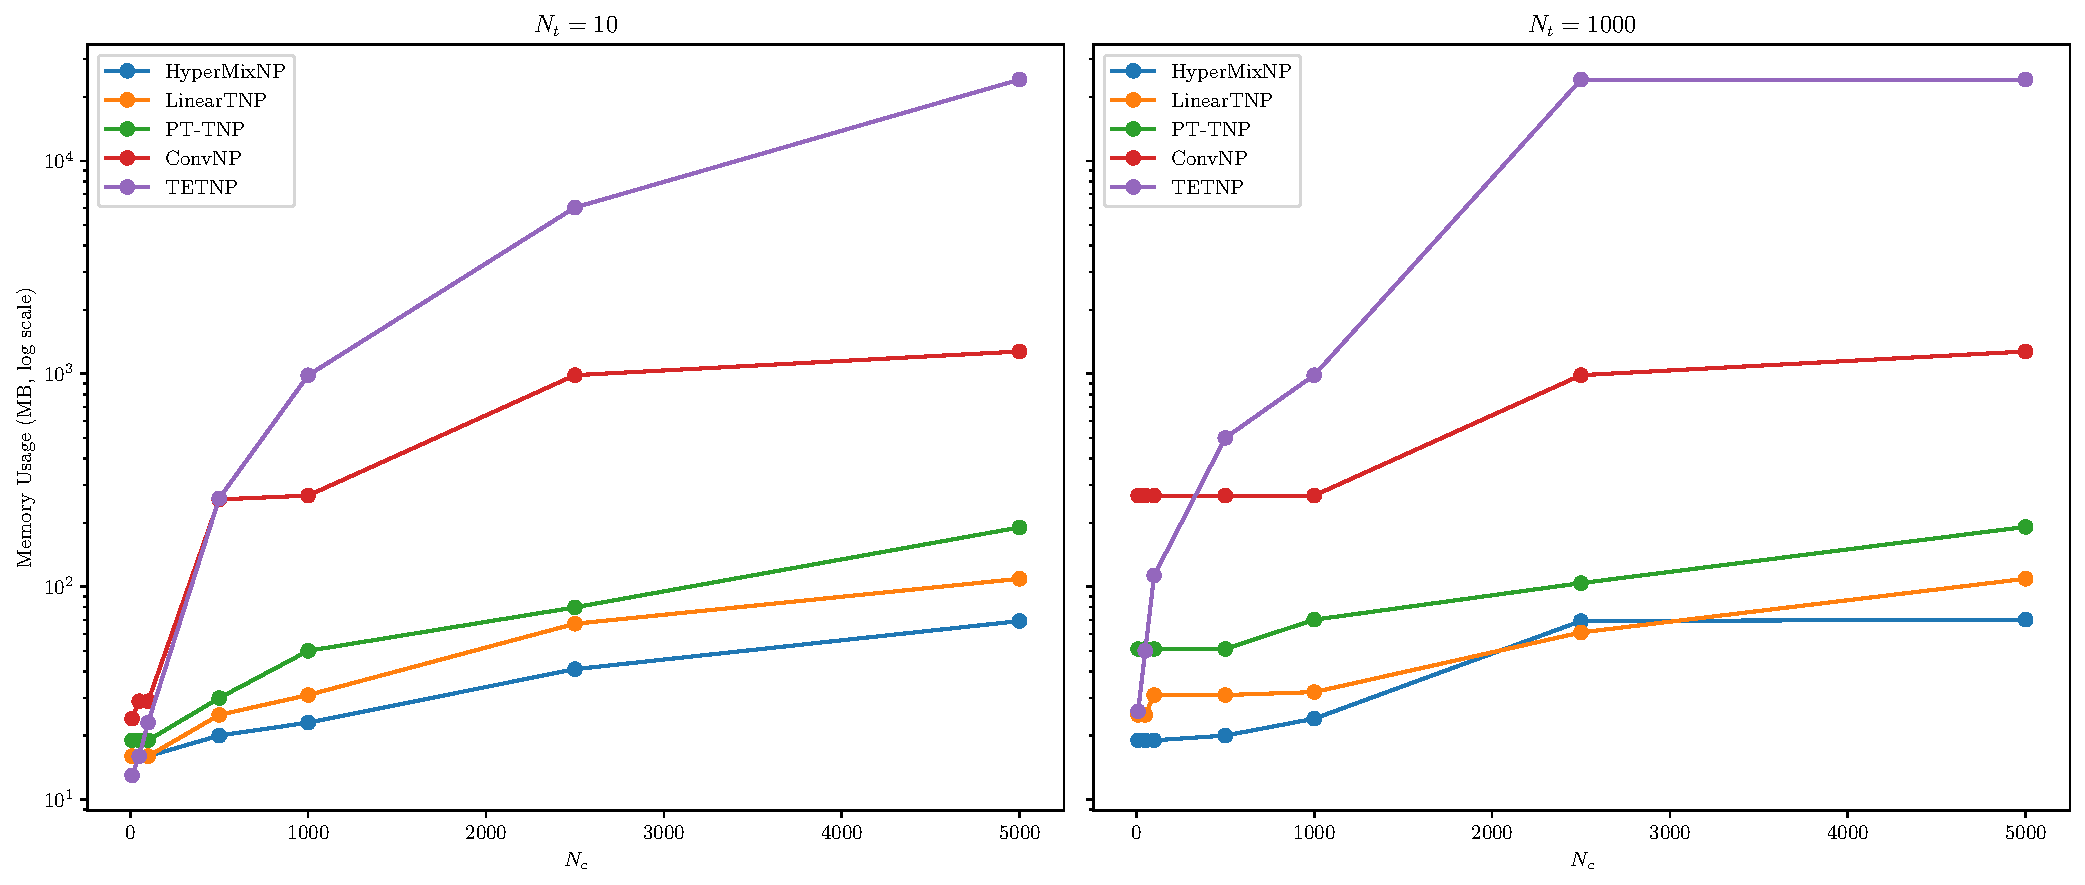
\includegraphics[width=0.97\textwidth]{fig/runtimelinear.pdf}
    \caption{Memory usage (MB) of the models on the 2D datasets using $N_t = 10$ (left) and $N_t = 1000$ (right). The $y$-axis is in log scale.}
    \label{fig:runtime-linear}
\end{figure}



\autoref{fig:runtime-linear} demonstrates the drastic improvement in memory usage of the linear models compared to the quadratic models. The linear models are able to scale to larger datasets with a much smaller memory footprint, making them suitable for large-scale applications where data is smooth, and the quadratic models are infeasible to use. 

\section{Summary}

The Linear Transformer models are a promising direction for scaling up the Transformer models to larger datasets. They were able to significantly reduce the memory complexity of the model, however the loss of performance on the Sawtooth dataset is concerning. More research is required to understand the limitations of the linear attention mechanism and potentially improve the performance of the models.



\ifSubfilesClassLoaded{%
    \printbibliography{}
}{} 


\end{document}